\section{Sprint 3 - System design}
After the completion of the third sprint we had arrived at a place where our application had most of the initial requirements implemented, or partially implemented. It presented itself in the following manner:
\newline
\newline
\begin{table}[h!]
\begin{center}
\begin{tabular}{cc}
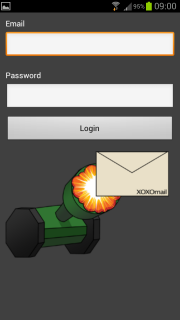
\includegraphics{logingui} & 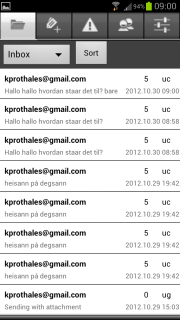
\includegraphics{inbox}
\end{tabular}
\end{center}
\caption{Login and inbox GUI} \label{tab:logininboxgui}
\end{table}

At first the user is prompted with a login screen where he has to type in his or hers username and password in order to get access to the application features. If the username and password is correct he/she is brought to the tabbed section of our application, more specifically the inbox tab. From the inbox tab the user is presented with a list of messages which he can sort after different criterias. He also has the ability to change between the inbox view and the sent messages view. If the user touches one of the messages displayed he is brought to the message view. See figure \ref{fig:viewmessagegui} at page \pageref{fig:viewmessagegui}.
\newline

\begin{figure}[h!]
\begin{center}
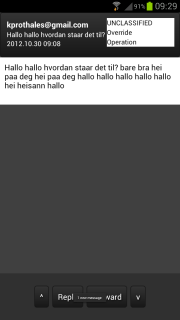
\includegraphics{viewmessage}
\end{center}
\caption{Message screen view} \label{fig:viewmessagegui}
\end{figure}

\newpage

From the \textsc{Message} view the user can see the message he selected. The title, message text, label, priority and type is shown to the user. From this view he can reply to the message, forward it and switch between received messages. See Figures in table \ref{tab:sendinstantmessage} at page \pageref{tab:sendinstantmessage}.
\newline
\begin{table}[h!]
\begin{center}
\begin{tabular}{cc}
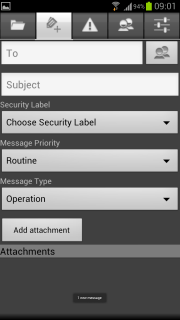
\includegraphics{sendmessage} & 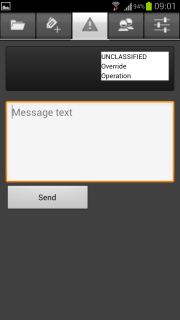
\includegraphics{instamessage}
\end{tabular}
\caption{Send message and Instant message GUI} \label{tab:sendinstantmessage}
\end{center}
\end{table}

If the user presses the second tab icon he is taken to the send message view. From here he can add a recipient either by entering the address manually or pressing the contacts icon and selecting a contact from a list that appears. He then types in a subject, selects label, priority and type. He also gets the ability to add an attachment to the message he is sending. 
\newline
\newline
When having pressed the third tab icon the user is brought to the instant message view. He he has the ability to send a message with predefined receiver, label, priority and type in a convenient way.
\newline
\begin{table}[h!]
\begin{center}
\begin{tabular}{cc}
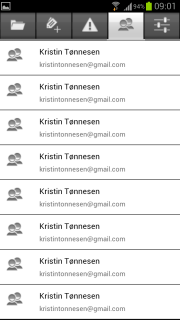
\includegraphics{contacts} & 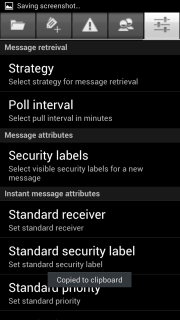
\includegraphics{settingsgui}
\end{tabular}
\end{center}
\caption{Contacts and Settings GUI} \label{tab:contactssetingsgui}
\end{table}

\newpage

If the fourth tab is selected the user is now viewing the contacts. This is the only functionality of this tab. 
\newline
\newline
When the fifth and final tab icon is selected the settings screen is showed to the user. From here the user can select the message retrieval strategy (either push or pull) as well as the poll interval for the pull implementation. He can also select the security labels that are presented to when sending a new message. The instant message standard fields are also selected from the settings menu along with some location data settings.   
\newline
\newline
The application has changed quite a bit since sprint two, it now has a more complete feel to it and new vital functionality has been added. See the firgures in table \ref{tab:contactssetingsgui} at page \pageref{tab:contactssetingsgui}.